\documentclass[a4paper,10pt,reqno]{amsart}

\makeatletter
\def\specialsection{\@startsection{section}{1}%
  \z@{\linespacing\@plus\linespacing}{.5\linespacing}%
  {\bfseries\centering}}
\def\section{\@startsection{section}{1}%
  \z@{.7\linespacing\@plus\linespacing}{.5\linespacing}%
  {\bfseries\scshape\centering}}
\makeatother

\newenvironment{nouppercase}{%
  \let\uppercase\relax%
  \renewcommand{\uppercasenonmath}[1]{}}{}


\usepackage[utf8]{inputenc}
\usepackage[foot]{amsaddr}
\usepackage{amsmath,amsfonts,amssymb,amsthm,mathrsfs,bm}
\usepackage[margin=0.7in]{geometry}
\usepackage{color}
\usepackage[dvipsnames]{xcolor}
\usepackage{multicol}
\usepackage{soul}
\usepackage{float}

\usepackage{etoolbox}

% Modifications to amsart ToC-related macros...
\makeatletter
\let\old@tocline\@tocline
\let\section@tocline\@tocline
% Insert a dotted ToC-line for \subsection and \subsubsection only
\newcommand{\subsection@dotsep}{4.5}
\newcommand{\subsubsection@dotsep}{4.5}
\patchcmd{\@tocline}
  {\hfil}
  {\nobreak
     \leaders\hbox{$\m@th
        \mkern \subsection@dotsep mu\hbox{.}\mkern \subsection@dotsep mu$}\hfill
     \nobreak}{}{}
\let\subsection@tocline\@tocline
\let\@tocline\old@tocline

\patchcmd{\@tocline}
  {\hfil}
  {\nobreak
     \leaders\hbox{$\m@th
        \mkern \subsubsection@dotsep mu\hbox{.}\mkern \subsubsection@dotsep mu$}\hfill
     \nobreak}{}{}
\let\subsubsection@tocline\@tocline
\let\@tocline\old@tocline

\let\old@l@subsection\l@subsection
\let\old@l@subsubsection\l@subsubsection

\def\@tocwriteb#1#2#3{%
  \begingroup
    \@xp\def\csname #2@tocline\endcsname##1##2##3##4##5##6{%
      \ifnum##1>\c@tocdepth
      \else \sbox\z@{##5\let\indentlabel\@tochangmeasure##6}\fi}%
    \csname l@#2\endcsname{#1{\csname#2name\endcsname}{\@secnumber}{}}%
  \endgroup
  \addcontentsline{toc}{#2}%
    {\protect#1{\csname#2name\endcsname}{\@secnumber}{#3}}}%

% Handle section-specific indentation and number width of ToC-related entries
\newlength{\@tocsectionindent}
\newlength{\@tocsubsectionindent}
\newlength{\@tocsubsubsectionindent}
\newlength{\@tocsectionnumwidth}
\newlength{\@tocsubsectionnumwidth}
\newlength{\@tocsubsubsectionnumwidth}
\newcommand{\settocsectionnumwidth}[1]{\setlength{\@tocsectionnumwidth}{#1}}
\newcommand{\settocsubsectionnumwidth}[1]{\setlength{\@tocsubsectionnumwidth}{#1}}
\newcommand{\settocsubsubsectionnumwidth}[1]{\setlength{\@tocsubsubsectionnumwidth}{#1}}
\newcommand{\settocsectionindent}[1]{\setlength{\@tocsectionindent}{#1}}
\newcommand{\settocsubsectionindent}[1]{\setlength{\@tocsubsectionindent}{#1}}
\newcommand{\settocsubsubsectionindent}[1]{\setlength{\@tocsubsubsectionindent}{#1}}

% Handle section-specific formatting and vertical skip of ToC-related entries
% \@tocline{<level>}{<vspace>}{<indent>}{<numberwidth>}{<extra>}{<text>}{<pagenum>}
\renewcommand{\l@section}{\section@tocline{1}{\@tocsectionvskip}{\@tocsectionindent}{}{\@tocsectionformat}}%
\renewcommand{\l@subsection}{\subsection@tocline{1}{\@tocsubsectionvskip}{\@tocsubsectionindent}{}{\@tocsubsectionformat}}%
\renewcommand{\l@subsubsection}{\subsubsection@tocline{1}{\@tocsubsubsectionvskip}{\@tocsubsubsectionindent}{}{\@tocsubsubsectionformat}}%
\newcommand{\@tocsectionformat}{}
\newcommand{\@tocsubsectionformat}{}
\newcommand{\@tocsubsubsectionformat}{}
\expandafter\def\csname toc@1format\endcsname{\@tocsectionformat}
\expandafter\def\csname toc@2format\endcsname{\@tocsubsectionformat}
\expandafter\def\csname toc@3format\endcsname{\@tocsubsubsectionformat}
\newcommand{\settocsectionformat}[1]{\renewcommand{\@tocsectionformat}{#1}}
\newcommand{\settocsubsectionformat}[1]{\renewcommand{\@tocsubsectionformat}{#1}}
\newcommand{\settocsubsubsectionformat}[1]{\renewcommand{\@tocsubsubsectionformat}{#1}}
\newlength{\@tocsectionvskip}
\newcommand{\settocsectionvskip}[1]{\setlength{\@tocsectionvskip}{#1}}
\newlength{\@tocsubsectionvskip}
\newcommand{\settocsubsectionvskip}[1]{\setlength{\@tocsubsectionvskip}{#1}}
\newlength{\@tocsubsubsectionvskip}
\newcommand{\settocsubsubsectionvskip}[1]{\setlength{\@tocsubsubsectionvskip}{#1}}

% Adjust section-specific ToC-related macros to have a fixed-width numbering framework
\patchcmd{\tocsection}{\indentlabel}{\makebox[\@tocsectionnumwidth][l]}{}{}
\patchcmd{\tocsubsection}{\indentlabel}{\makebox[\@tocsubsectionnumwidth][l]}{}{}
\patchcmd{\tocsubsubsection}{\indentlabel}{\makebox[\@tocsubsubsectionnumwidth][l]}{}{}

% Allow for section-specific page numbering format of ToC-related entries
\newcommand{\@sectypepnumformat}{}
\renewcommand{\contentsline}[1]{%
  \expandafter\let\expandafter\@sectypepnumformat\csname @toc#1pnumformat\endcsname%
  \csname l@#1\endcsname}
\newcommand{\@tocsectionpnumformat}{}
\newcommand{\@tocsubsectionpnumformat}{}
\newcommand{\@tocsubsubsectionpnumformat}{}
\newcommand{\setsectionpnumformat}[1]{\renewcommand{\@tocsectionpnumformat}{#1}}
\newcommand{\setsubsectionpnumformat}[1]{\renewcommand{\@tocsubsectionpnumformat}{#1}}
\newcommand{\setsubsubsectionpnumformat}[1]{\renewcommand{\@tocsubsubsectionpnumformat}{#1}}
\renewcommand{\@tocpagenum}[1]{%
  \hfill {\mdseries\@sectypepnumformat #1}}

% Small correction to Appendix, since it's still a \section which should be handled differently
\let\oldappendix\appendix
\renewcommand{\appendix}{%
  \leavevmode\oldappendix%
  \addtocontents{toc}{%
    \protect\settowidth{\protect\@tocsectionnumwidth}{\protect\@tocsectionformat\sectionname\space}%
    \protect\addtolength{\protect\@tocsectionnumwidth}{2em}}%
}
\makeatother

% #1 (default is as required)

% #2

% #3
\makeatletter
\settocsectionnumwidth{2em}
\settocsubsectionnumwidth{2.5em}
\settocsubsubsectionnumwidth{3em}
\settocsectionindent{1pc}%
\settocsubsectionindent{\dimexpr\@tocsectionindent+\@tocsectionnumwidth}%
\settocsubsubsectionindent{\dimexpr\@tocsubsectionindent+\@tocsubsectionnumwidth}%
\makeatother

% #4 & #5
\settocsectionvskip{10pt}
\settocsubsectionvskip{0pt}
\settocsubsubsectionvskip{0pt}

% #6 & #7
% See #3

% #8
\renewcommand{\contentsnamefont}{\bfseries\Large}

% #9
\settocsectionformat{\bfseries}
\settocsubsectionformat{\mdseries}
\settocsubsubsectionformat{\mdseries}
\setsectionpnumformat{\bfseries}
\setsubsectionpnumformat{\mdseries}
\setsubsubsectionpnumformat{\mdseries}

% #10
% Insert the following command inside your text where you want the ToC to have a page break
\newcommand{\tocpagebreak}{\leavevmode\addtocontents{toc}{\protect\clearpage}}

% #11
\let\oldtableofcontents\tableofcontents
\renewcommand{\tableofcontents}{%
  \vspace*{-\linespacing}% Default gap to top of CONTENTS is \linespacing.
  \oldtableofcontents}

\usepackage{mathtools,enumerate,mathrsfs,graphicx}
\usepackage{epstopdf}
\usepackage{hyperref}
\usepackage{latexsym}
\usepackage{graphicx}
\usepackage{subcaption}
\usepackage{tcolorbox}


\definecolor{CommentGreen}{rgb}{0.0,0.4,0.0}
\definecolor{Background}{rgb}{0.9,0.9,09}
\definecolor{lrow}{rgb}{0.914,0.918,0.922}
\definecolor{drow}{rgb}{0.725,0.745,0.769}
\definecolor{darkGreen}{RGB}{38,178,0}

\usepackage{listings}
\usepackage{textcomp}
\lstloadlanguages{Matlab}%
\lstset{
    language=Matlab,
    upquote=true, frame=single,
    basicstyle=\small\ttfamily,
    backgroundcolor=\color{Background},
    keywordstyle=[1]\color{blue}\bfseries,
    keywordstyle=[2]\color{purple},
    keywordstyle=[3]\color{black}\bfseries,
    identifierstyle=,
    commentstyle=\usefont{T1}{pcr}{m}{sl}\color{CommentGreen}\small,
    stringstyle=\color{purple},
    showstringspaces=false, tabsize=5,
    morekeywords={properties,methods,classdef},
    morekeywords=[2]{handle},
    morecomment=[l][\color{blue}]{...},
    numbers=none, firstnumber=1,
    numberstyle=\tiny\color{blue},
    stepnumber=1, xleftmargin=10pt, xrightmargin=10pt
}

\numberwithin{equation}{section}
\synctex=1

\hypersetup{
    unicode=false, pdftoolbar=true, 
    pdfmenubar=true, pdffitwindow=false, pdfstartview={FitH}, 
    pdftitle={ELE2024 Coursework}, pdfauthor={A. Author},
    pdfsubject={ELE2024 coursework}, pdfcreator={A. Author},
    pdfproducer={ELE2024}, pdfnewwindow=true,
    colorlinks=true, linkcolor=red,
    citecolor=blue, filecolor=magenta, urlcolor=cyan
}


% CUSTOM COMMANDS
\renewcommand{\Re}{\mathbf{re}}
\renewcommand{\Im}{\mathbf{im}}
\newcommand{\R}{\mathbb{R}}
\newcommand{\N}{\mathbb{N}}
\newcommand{\C}{\mathbb{C}}
\newcommand{\lap}{\mathscr{L}}
\newcommand{\dd}{\mathrm{d}}
\newcommand{\smallmat}[1]{\left[ \begin{smallmatrix}#1 \end{smallmatrix} \right]}

%opening
\title[ELE2024 Coursework]{\Huge ELE2024 Control Coursework}

\author[T. Hagan]{\Large Created by Toby Hagan}
\author[L. Quail]{\Large Lorcán Quail}

\address[T. Hagan, L. Quail and S. Ullah]{. Email addresses: \href{mailto:thagan03@qub.ac.uk}%
{thagan03@qub.ac.uk},
\href{mailto:lquail02@qub.ac.uk}{lquail02@qub.ac.uk} and \href{mailto:sullah02@qub.ac.uk}{sullah02@qub.ac.uk}}
\thanks{
        Version 2.0.1. Last updated:~\today.}
\begin{document}

\begin{nouppercase}
\maketitle
\end{nouppercase}

\section*{Introduction}

\par Throughout this project, the nature of a system of a wooden ball on an inclined plane connected to a spring and attracted to an electromagnet was investigated. This system is outlined in figure~\ref{fig:A1Diagram}. For part B of this project, Python was used to simulate the experiments performed on the system and the code used is within this \href{https://github.com/Lorcan-Q/Control_Coursework}{Github repository}.

\begin{figure}[h]
 \centering
 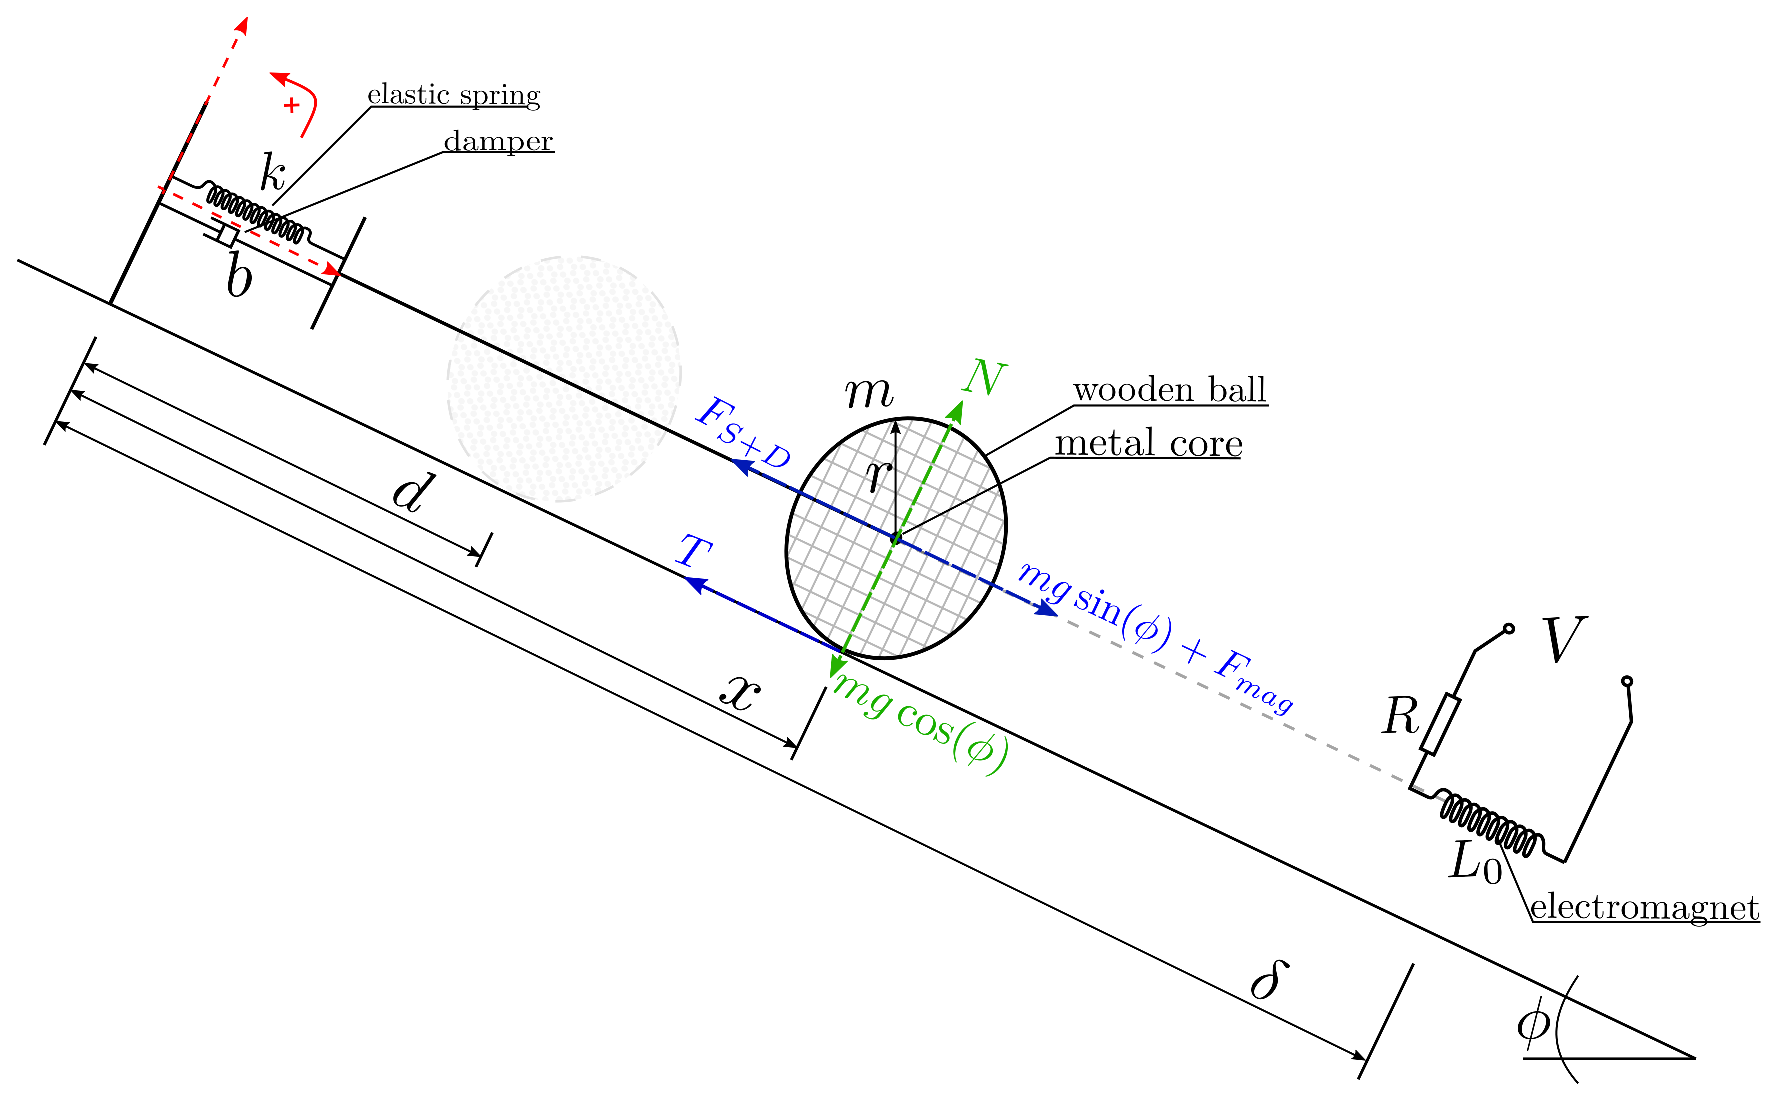
\includegraphics[width=0.6\linewidth]{Figures/FreeBody.eps}
 \caption{System of the wooden ball on an inclined plane with first principles applied.}
 \label{fig:A1Diagram}
\end{figure}

\section{Part A}

\subsection{A1 - System Modelling}\label{sec:A1}
To enable the system to be modeled as a set of ordinary differential equations, first principles are applied to the system. Obtaining equations requires the forces acting on the wooden ball be resolved; therefore the vertical forces, i.e. forces acting perpendicular to the slope, can be modelled as:

\begin{equation}
    \color{darkGreen}{N-mg\cos{\phi}=0}\color{black}
\end{equation}

The forces working parallel to the slope can be modelled as:

\begin{equation}
\label{eqn:ForcesOrg}
    \color{blue}{mg\sin{\phi}+F_{mag}-T-F_{S+D}=m\ddot{x}}\color{black}
\end{equation}

Where \color{blue}{$F_{mag}$} \color{black}and \color{blue}{$F_{S+D}$} \color{black}are defined as:
\begin{align*}
    F_{mag} = c\bigg(\frac{I}{\delta-x}\bigg)^2
    && F_{S+D}=k(x-d)+b\dot{x}\\
\end{align*}
\par The static friction, \color{blue}{$T$}\color{black}, can be resolved utilizing the equation for the torque created on the ball:
\begin{align}
    Torque(M)&{}={}-Tr=I\ddot{\theta}
    \notag\\
    T &= \frac{-I\ddot{\theta}}{r}
    \label{eqn:torque}
\end{align}
\par As the ball rotates contrary to the counter-clockwise direction which is taken as positive, the torque is defined in the negative direction. 


\newpage
The equation defining the length or a given arc of a circle is defined as $x=r(\theta)$. However, as counter-clockwise rotations are taken as negative in the model and the ball rotates clockwise, the equation results in  $x=r(-\theta)$. Differentiating this equation results in, $\ddot{\theta}=\frac{\ddot{-x}}{r}$. Furthermore, the moment of inertia for the solid ball is defined as $I=\frac{2mr^2}{5}$. Thus, the static friction can be defined as:
\begin{align}
    T=-\frac{1}{r}\bigg(\frac{2mr^2}{5}\bigg)\bigg(\frac{-\ddot{x}}{r}\bigg)
    \notag\\
    T = \frac{2mr^2\ddot{x}}{5R^2} = \frac{2m\ddot{x}}{5}
\end{align}
\\
\par The resolved forces are inputted into equation~\ref{eqn:ForcesOrg} to obtain:
\begin{align}
    m\ddot{x} &{}={} mg\sin{\phi}+c[\frac{I}{\delta-x}]^2-\frac{2m\ddot{x}}{5}-k(x-d)-b\dot{x}
    \notag
    \\
    \frac{7m\ddot{x}}{5} &{}={} mg\sin{\phi}+c(\frac{I}{\delta-x})^2-k(x-d)-b\dot{x}
    \label{eqn:non-linear x}
\end{align}
\\
\par To describe how the input voltage $V$ affects the position $x$ of the ball on the inclined plane, an equation for how the electromagnet behaves can be derived. This is achieved using, $V_{in}=V_R+V_L$, $V_R=RI$ and $V_L=L\dot{I}$
\begin{align}
    V_L&{}={}V_{in}-V_R
    \notag\\
    L\dot{I}&{}={}V-RI
    \notag\\
    \dot{I}&{}={}\frac{1}{L}(V-RI)
    \label{eqn:non-linear I}
\end{align}
where $L$ is defined as $L= L_0 +L_1e^{-\alpha(\delta-x)}$
\\


The dynamics of the system can be described by the following ordinary differential equations (\ref{eqn:non-linear x}, \ref{eqn:non-linear I}):
\begin{subequations}\label{eqn:non-linear sys}
\begin{align} 
    \ddot{x}&{}={}\frac{5}{7m}\bigg(mg\sin{\phi}+c[\frac{I}{\delta-x}]^2-k(x-d)-b\dot{x}\bigg)
    \\
    \dot{I}&{}={}\frac{1}{L_O+L_1e^{-\alpha(\delta-x)}}(V-RI)
    \\
    \notag
\end{align}
\end{subequations}
\subsection{A2 - State Space Representation}\label{sec:A2}
\par Modelling the system in the state space representation will describe the system in terms of its states and inputs. As the model involves terms that are non-linear, utilising the state space representation will enable the linearisation of these terms to be preformed. State variables are created to reduce the ordinary differential equations to the first-order:

\begin{equation}
\label{eqn:state vars}
\bm{z}=
\begin{bmatrix}
z_1
\\
z_2
\\
z_3
\end{bmatrix}
=
\begin{bmatrix}
x
\\
\dot{x}
\\
I
\end{bmatrix}
\end{equation}
\\

Inserting the state variables (\ref{eqn:state vars}), into the system equations (\ref{eqn:non-linear sys}) 
\begin{equation}
    \dot{z_2}=\frac{5}{7m}(mg\sin{\phi}+c[\frac{z_3}{(\delta-z_1)}]-k(z_1-d)-bz_2)
    \label{eqn:non-linear z_2}
\end{equation}
\begin{equation}
    \dot{z_3}=\frac{V-z_3R}{L_o+L_1e^{-\alpha(\delta-x)}}
    \label{eqn:non-linear z_3}
\end{equation}
\\
The state space representation is defined below, with states $z1, z2, z3$ (defined in \ref{eqn:state vars}) and input V;

\begin{equation}\label{eqn:ssr}
\bm{\dot{z}}=
\begin{bmatrix}
\dot{z_1}
\\
\dot{z_2}
\\
\dot{z_3}
\end{bmatrix}
=
\begin{bmatrix}
z_2
\\
\frac{5}{7m}(mg\sin{\phi}+c[\frac{z_3}{(\delta-z_1}]-k(z_1-d)-bz_2)
\\
\frac{V-z_3R}{L_o+L_1e^{-\alpha(\delta-x)}}
\end{bmatrix}
\end{equation} 
\\
\newpage
\subsection{A3 - Characterisation of the Equilibrium Points.}\label{sec:A3} 

\par The state space representation (\ref{eqn:ssr}) enables the equilibrium points of the system to be characterised. A state-input pair ($z^e, v^e$) is defined as an equilibrium point of the system providing that $f(z^e,v^e)=0$:
\begin{subequations}\label{eqn:Charaterised EQ}
\begin{gather}
    0=z_2^e \label{eqn:z_2^e=0}
    \\
    0=\frac{5}{7m}\bigg(mg\sin{\phi}+\frac{c(z_3^e)^2}{(\delta-z_1^e)^2}-k(z_1^e-d)-z_2^e\bigg)
    \\\
    0=\frac{V^e-z_3^eR}{L_o+L_1e^{-\alpha(\delta-z_1^e)}}\label{eqn:V^e=I^eR}
\end{gather}
\end{subequations}
\\
\par It is important to note that at equilibrium the ball would be stationary, this is shown in equation \ref{eqn:z_2^e=0}. Furthermore, equation \ref{eqn:V^e=I^eR} demonstrates that at equilibrium, $V^e=z_3^eR$.

\subsection{A4 - System Linearisation}\label{sec:A4}
\par Following the characterisation of the equilibrium points, this enables the non-linear system to be linearised through the linear approximation of its non-linear terms. In order to remove the constant terms, subtracting by parts the state space equations (\ref{eqn:ssr}) from their characterised equilibrium points (\ref{eqn:Charaterised EQ}):
\begin{subequations}
\begin{gather}
    \dot{z_1}=z_2-z_2^e
    \\
    \dot{z_2} = \frac{5}{7m}\bigg(mg\sin{\phi}+\frac{cz_3^2}{(\delta-z_1)^2}-k(z_1-d)-bz_2\bigg)-\frac{5}{7m}\bigg(mg\sin{\phi}+\frac{c(z_3^e)^2}{(\delta-z_1^e)^2}-k(z_1^e-d)\bigg)
    \label{eqn:z_2}\\
    \dot{z_3}=\frac{V-z_3R}{L_o+L_1e^{-\alpha(\delta-z_1)}}-\frac{V^e-z_3^eR}{L_o+L_1e^{-\alpha(\delta-z_1^e)}}
\end{gather}
\end{subequations}
\\
\par This enables the constant terms present in \ref{eqn:z_2} to be removed producing:
\begin{subequations}
\begin{gather}
    \dot{z_1}=z_2-z_2^e
    \\
    \dot{z_2} = \frac{5}{7m}\bigg[c\bigg(\Psi_1(z_3,z_1)-\frac{(z_3^e)^2}{(\delta-z_1^e)^2}\bigg)-k(z_1-z_1^e)-bz_2\bigg]
    \\
    \dot{z_3}=\Psi_2(V, z_3,z_1)-\frac{V^e-z_3^eR}{L_o+L_1e^{-\alpha(\delta-z_1^e)}}
\end{gather}
\end{subequations}

Where:
\begin{align*}
    \Psi_1(z_3,z_1) = \frac{z_3^2}{(\delta-z_1)^2} 
    && \Psi_2(V, z_3,z_1) = \frac{V-z_3R}{L_o+L_1e^{-\alpha(\delta-z_1)}}
\end{align*}

\par To linearise the system the non-linear terms defined by $\Psi_1$ and $\Psi_2$ must be linearised at equilibrium.
The best linear approximation theorem derived from Taylor's approximation enables a good approximation of these terms providing that their state values are close to their values at equilibrium:
\begin{gather}
    \phi(x, y) {}\approx{} \phi(x^e, y^e)+ \frac{\partial \phi}{\partial x}\Bigg\rvert_{x^e,y^e}(x-x^e)+\frac{\partial \phi}{\partial y}\Bigg\rvert_{x^e,y^e}(y-y^e)
    \label{eqn:BLA}
\end{gather}
Hence, using the best approximation theorem (\ref{eqn:BLA}) on the non-linear terms:
\begin{align*}
    \Psi_1(z_3,z_1)&=\frac{z_3^2}{(\delta-z_1)^2}\approx\Psi_1(z_3^e,z_1^e)+\frac{\partial\Psi_1}{\partial z_3}\Bigg\rvert_{z_3^e,z_1^e}(z_3-z_3^e)+\frac{\partial\Psi_1}{\partial z_1}\Bigg\rvert_{z_3^e,z_1^e}(z_1-z_1^e)
\end{align*}
Where,
\begin{align*}
    \frac{\delta\Psi_1}{\delta z_3}\Bigg\rvert_{z_3^e,z_1^e}=\frac{2z_3^e}{(\delta-z_1^e)^2}
    && 
    \frac{\delta\Psi_1}{\delta z_1}\Bigg\rvert_{z_3^e,z_1^e}=\frac{(z_3^e)^2}{(\delta-z_1^e)^3}
\end{align*}
Hence,
\begin{align}\label{eqn:Phi_1 lin}
    \Psi_1(z_3,z_1) - \Psi_1(z_3^e,z_1^e) \approx \frac{2z_3^e}{(\delta-z_1^e)^2}(z_3-z_3^e) + \frac{(z_3^e)^2}{(\delta-z_1^e)^3}(z_1-z_1^e)
\end{align}

\begin{align*}
    \Psi_2(V,z_3,z_1)\approx\Psi_2(V^e,z_3^e,z_1^e)+\frac{\partial\Psi_2}{\partial V}\Bigg\rvert_{V^e, z_3^e,z_1^e}(V-V^e)+\frac{\partial\Psi_2}{\partial z_3}\Bigg\rvert_{V^e, z_3^e,z_1^e}(z_3-z_3^e)+\frac{\partial\Psi-2}{\partial z_1}\Bigg\rvert_{V^e,z_3^e,z_1^e}(z_1-z_1^e)
\end{align*}
Where,
\begin{align*}
    \frac{\delta\Psi_2}{\delta V}\Bigg\rvert_{z_3^e,z_1^e} = \frac{1}{L_0+L_1e^{-\alpha(\delta-z_1^e)}}
    &&\frac{\delta\Psi_2}{\delta z_3}\Bigg\rvert_{z_3^e,z_1^e}=\frac{-R}{L_0+L_1e^{-\alpha(\delta-z_1^e)}}
    &&\frac{\delta\Psi_2}{\delta z_1}\Bigg\rvert_{z_3^e,z_1^e}=\frac{-\alpha L_1e^{-\alpha(\delta-z_1^e)}(V^e-z_3^eR)}{(L_0+L_1e^{-\alpha(\delta-z_1^e)})^2}
\end{align*}
   
As demonstrated in section \ref{sec:A3}, $V^e=z_3^eR$ hence the final partial derivative equates to zero:
\begin{align}\label{eqn:Phi_2 lin}
    \Psi_2(V, z_3, z_1) - \Psi_2(V^e,z_3^e,z_1^e) \approx \frac{1}{L_0+L_1e^{-\alpha(\delta-z_1^e)}}(V-V^e) + \frac{-R}{L_0+L_1e^{-\alpha(\delta-z_1^e)}}(z_3-z_3^e) + 0
\end{align}
To simplify the expressions, deviation variables are introduced: 
\begin{align}\label{eqn:Deviation}
    \bar{z_1} = z_1 - z_1^e && \bar{z_2} = z_2 - z_2^e && \bar{z_3}=z_3-z_3^e && \bar{V}=V-V^e
\end{align}
The linearised equations can be defined using the linearisation of the non-linear terms (\ref{eqn:Phi_1 lin}, \ref{eqn:Phi_2 lin}) and the deviation variables (\ref{eqn:Deviation}):
\begin{subequations}\label{eqn:lin_eqs}
\begin{align}
    \dot{z_2}&=\frac{5c}{7m}\bigg(\frac{2z_3^e}{(\delta-z_1^e)^2}(\bar{z_3})+\frac{2(z_3^e)^2}{(\delta-z_1^e)^3}(\bar{z_1})\bigg)-\frac{5k}{7m}(\bar{z_1})-\frac{5b}{7m}(\bar{z_2})
    \notag\\
    &=\frac{10cz_3^e}{7m(\delta-z_1^e)^2}(\bar{z_3})+\frac{10c(z_3^e)^2}{7m(\delta-z_1^e)^3}(\bar{z_1})-\frac{5k}{7m}(\bar{z_1})-\frac{5b}{7m}(\bar{z_2})
    \notag\\
    &=\frac{10cz_3^e}{7m(\delta-z_1^e)^2}(\bar{z_3})+\frac{5}{7m}\bigg(\frac{2c(z_3^e)^2}{(\delta-z_1^e)^3}-k\bigg)(\bar{z_1})-\frac{5b}{7m}(\bar{z_2})
    \notag
    \\
    &=\color{red}a_1\color{black}\bar{z_3} + \color{red}a_2\color{black}\bar{z_1} - \color{red}a_3\color{black}\bar{z_2}
\\
\notag
\\
    \dot{z_3}&=\frac{\bar{V}}{L_o+L_1^{-\alpha(\delta-z_1)}}-\frac{R\bar{z_3}}{L_o+L_1^{-\alpha(\delta-z_1^e)}}
    \notag\\
    &=\frac{1}{L_o+L_1e^{\alpha(z_1^e-\delta)}}(\bar{V}-R\bar{z_3})
    \notag\\
    &=\color{red}a_4\color{black}(\bar{V}-R\bar{z_3})
\end{align}
\end{subequations}
Where,
\begin{align}\label{eqn:lin_vars}
    \color{red}a_1\color{black}=\frac{10cz_3^e}{7m(\delta-z_1^e)^2} && 
    \color{red}a_2\color{black}=\frac{5}{7m}\bigg(\frac{2c(z_3^e)^2}{(\delta-z_1^e)^3}-k\bigg) &&
    \color{red}a_3\color{black}=\frac{5b}{7m} &&
    \color{red}a_4\color{black}=\frac{1}{L_o+L_1^{-\alpha(\delta-z_1^e)}}
\end{align}
Thus, the linearised system can be defined using equations \ref{eqn:lin_eqs} and \ref{eqn:lin_vars}:
\begin{subequations}
\begin{align}
    \bar{\dot{z_1}} &= \bar{z_2}
    \\
    \bar{\dot{z_2}} &= a_1\bar{z_3} + a_2\bar{z_1} - a_3\bar{z_2}
    \\
    \bar{\dot{z_3}} &= a_4(\bar{V}-R\bar{z_3})
\end{align}
\end{subequations}

\subsection{A5 - Transfer function of linearised system}\label{sec:A5} 

\par The transfer function of the system enables the system to be simulated for a given input. The state variable of interest is $z_1$ which co-responds to the position of the ball on the inverted plane, thus the transfer will describe this position of the ball for a given input voltage, V. To obtain the transfer function, the Laplace transform
\begin{subequations}
\begin{align}
    s\bar{Z_1}(s) &{}={} s\bar{Z_2}(s)\label{eqn:barZ_1(s)}
    \\
    s\bar{Z_2}(s) &{}={} a_1\bar{Z_3}+a_2\bar{Z_1}-a_3\bar{Z_2}\label{eqn:barZ_2(s)}
    \\
     s\bar{Z_3}(s) &{}={} a_4\bar{V}-a_4R\bar{Z_3}\label{eqn:barZ_3(s)}
\end{align}
\end{subequations}
Inserting the definition for $Z_2(s)$ from \ref{eqn:barZ_1(s)} into \ref{eqn:barZ_2(s)}:
\begin{align}
    s(s\bar{Z_1}(s)) &{}={} a_1\bar{Z_3}(s)+a_2\bar{Z_1}(s)-a_3\bar{Z_2}(s)\notag
    \\
    \bar{Z_3}(s) &{}={} \frac{\bar{Z_1}(s)(s^2+a_3s-a_2)}{a_1}\label{eqn:barZ_3(s):Z_1}
\end{align}
\\
Therefore, inserting equation \ref{eqn:barZ_3(s):Z_1} into equation \ref{eqn:barZ_3(s)} obtains:
\begin{equation}
    \frac{\bar{Z_1}}{\bar{V}}=\frac{a_1a_4}{(s+a_4R)(s^2+a_3s-a_2)}\color{red}= G_x\color{black}
\end{equation}
\\

\par This is a third-order transfer function, thus has three poles. This can be modelled using the product of a first and second order transfer function for analytical purposes. Furthermore, the system's response can be approximated using the sum of the responses from the decomposed functions.

\begin{equation}
    G_x = a_1a_4\cdot\bigg(\frac{1}{s+a_4R}\bigg)\bigg(\frac{1}{s^2+a_3s-a_2}\bigg)
\end{equation}

\par Due to the nature of the summation, oscillations present in an impulse reaction from the second-order system would become apparent in the overall system's impulse response. These oscillations would be created due to the second order system being under-damped.
\\
\par A second order transfer function has the form:
\begin{equation}
    G(s) = \frac{k}{\tau^2s^2+2\zeta\tau s+1}
\end{equation}
where $k$, $\tau$, $\zeta >$ 0 and $k$ is the static gain, $\zeta$ is the damping factor and $\tau$ is the time constant of the system.
\par An under-damped second order system is categorised by a pair of complex, conjugate, non-real poles. The nature of the poles can be identified by analysing the discriminant of the denominator.
\begin{align*}
    \Delta\tau^2s^2+2\zeta\tau s+1&=(2\zeta\tau)^2 - 4(\tau^2)(1)
    \\
    &=4\zeta^2\tau^2-4\tau^2
    \\
    &=4\tau^2(\zeta^2-1)
\end{align*}

Hence, a damping factor $0 < \zeta < 1$, would create a negative discriminant indicating the system is under-damped due to the presence of a pair of non-real conjugate poles.
\\
\par Equating the second-order transfer function's co-coefficients produces:
\begin{align*}
    \tau^2=1 && 2\zeta\tau&=a_3
    \\
    && \zeta &= \frac{5b}{7m} \cdot \frac{1}{2} = \frac{5b}{14m}
\end{align*}

\par The system would present oscillations from an impulse response given that:
\begin{equation*}
    0 < \frac{5b}{14m} < 1
\end{equation*}
\\
\section{Part B}

\subsection{B1 - Equilibrating system at $x^e$}

%overleaf has an issue with equilibrate however it seems fine to me
\par Due to the forces acting on the system, the ball is only able to equilibrate within a defined space along the plane; utilising the characterised equilibrium points defined in section~\ref{sec:A3}, this space can be defined:

\begin{gather*}
    0=\frac{V^e-z_3^eR}{L_o+L_1^{-\alpha(\delta-z_1^e)}} \rightarrow V^e = z_3^eR
    \\
    0 = \frac{5}{7m}\bigg[mg\sin{\phi}+\frac{c(z_3^e)^2}{(\delta-z_1^e)^2}-k(z_1^e-d)\bigg]
    \\
    0 = mg\sin{\phi}(\delta-z_1^e)^2 + c(z_3^e)^2 - k(z_1^e-d)(\delta-z_1^e)^2
    \\
    z_3^e = \frac{(\delta-z_1^e)(k(z_1^e-d)-mg\sin{\phi})^\frac{1}{2}}{\sqrt{c}}
\end{gather*}

\par Therefore:

\begin{equation}
\label{eqn:V^e}
    V^e = \frac{R(\delta-z_1^e)(k(z_1^e-d)-mg\sin{\phi})^\frac{1}{2}}{\sqrt{c}}
\end{equation}
\\
\par Evidently from these equations, inputting a value of $z_1^e(x^e) \leq (\frac{mg\sin{\phi}}{k}+d)$ would result in the voltage and current resulting in a zero or imaginary value. Furthermore, a value of $z_1^e(x^e) \geq d$ would create a zero or negative result for the equilibrium values which indicate that the electromagnet polarity has switched, thus the ball would not achieve equilibrium. These derivations enable the space to be defined as:
\begin{equation}
    x_{min} < x^e < x_{max}
\end{equation}
 Where $x_{min} = d + \frac{mg\sin{\phi}}{k}$ and $x_{max} = \delta$

\newpage
\par Furthermore, using equation~\ref{eqn:V^e}, the ball's equilibrium position at which the equilibrium voltage attains a maximum can be determined.
\begin{figure}[h]
 \centering
 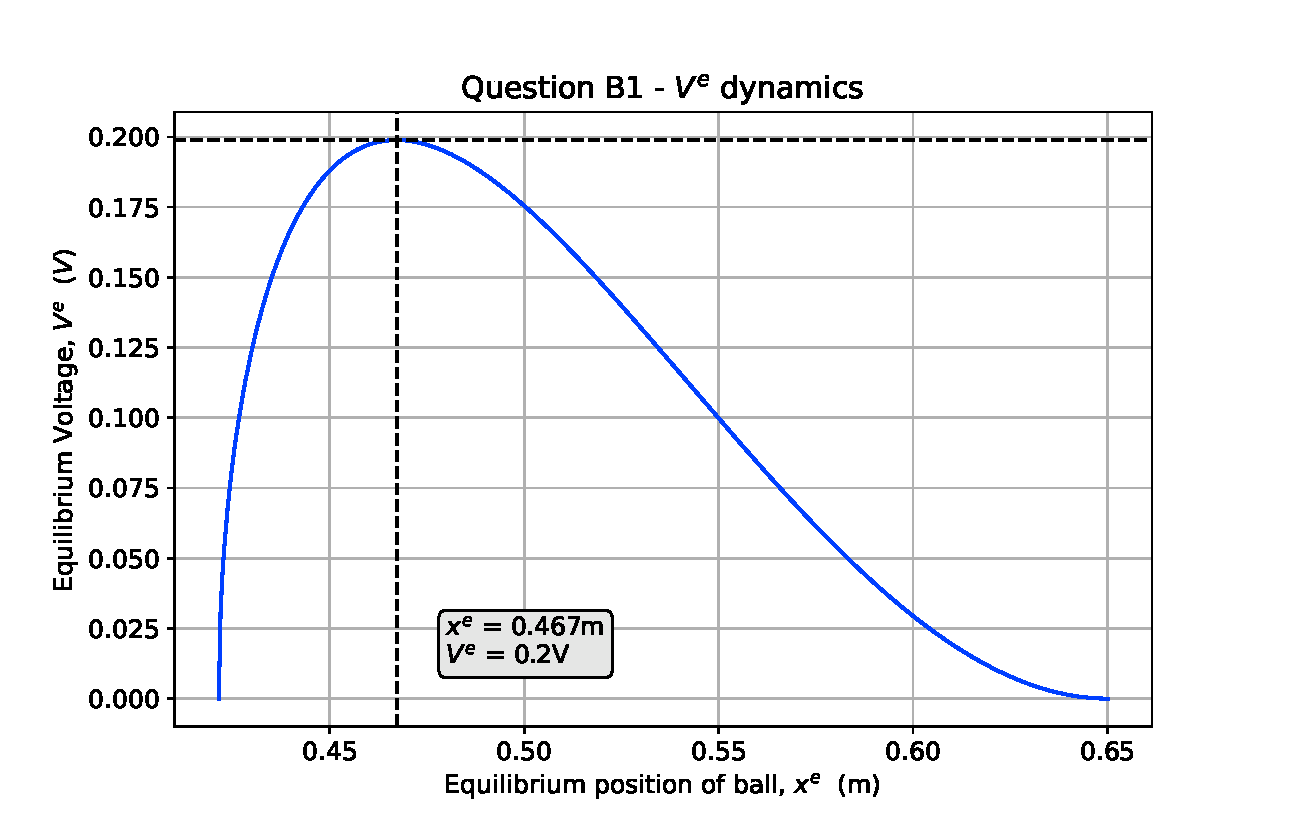
\includegraphics[width=0.6\linewidth]{Figures/B1.eps}
 \caption{Nature of the equilibrium values of $x^e$ and $V^e$ in the system using equation~\ref{eqn:V^e} when simulated in Python.}
 \label{fig:B1Diagram}
\end{figure}
\par As presented in figure~\ref{fig:B1Diagram}, the maximum voltage is approximately equal to 0.2 volts where the equilibrium position is equal to 0.467 metres.

\subsection{B2 - Verifying system linearisation through simulation}

\par Within this section, a program was developed in Python to simulate both the linear and non-linear dynamical systems determined in section~\ref{sec:A2}. During this section, the input voltage is equal to $V^e$ for all $t\geq0$ and the initial state of the system is close to its equilibrium value.

\begin{figure}[h]
\begin{subfigure}{.5\linewidth}
    \centering
    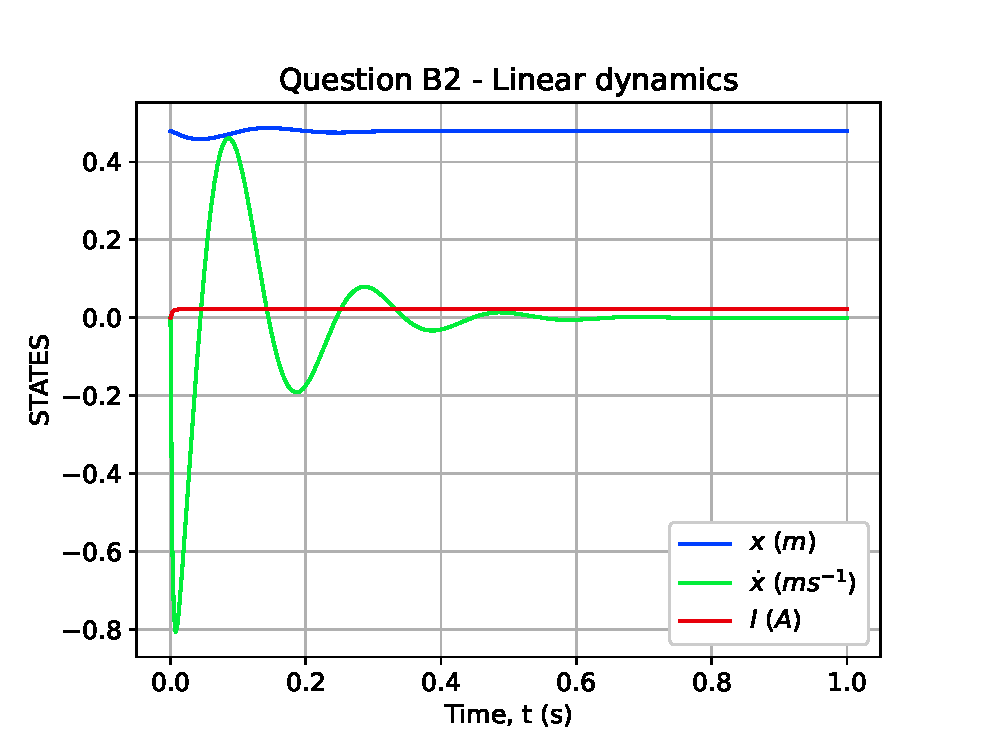
\includegraphics[width=1\linewidth]{Figures/B2_Linear.eps}
    \caption{Simulation of the non-linear system (defined by ~\ref{eqn:non-linear sys}).}
    \label{fig:B2LDiagram}
\end{subfigure}%
\begin{subfigure}{.5\linewidth}
    \centering
    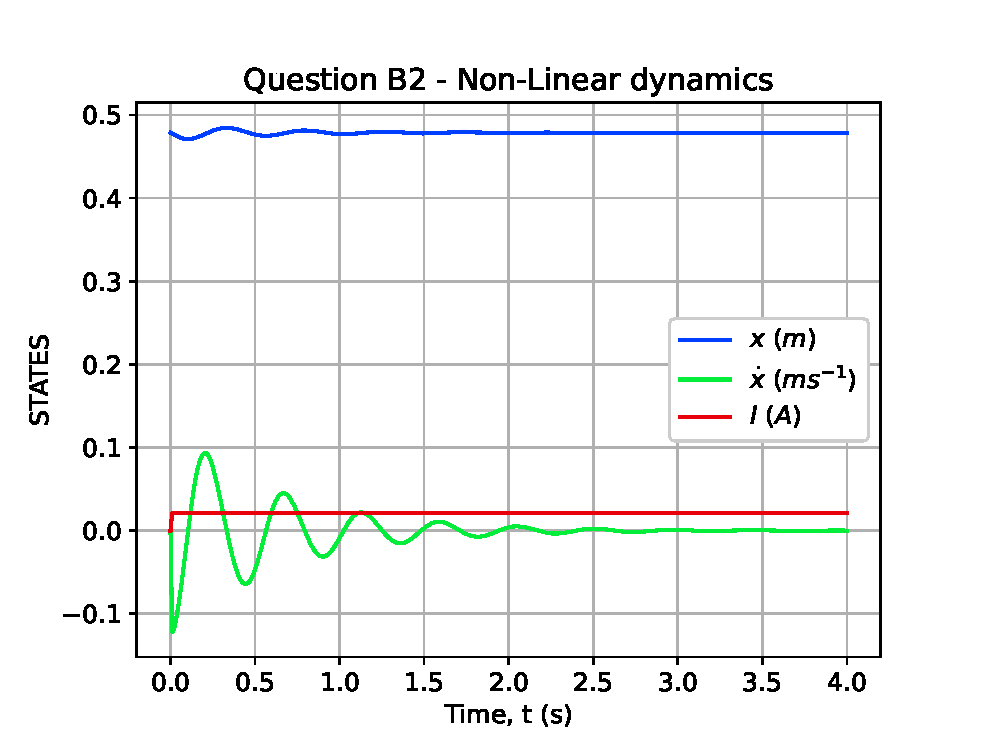
\includegraphics[width=1\linewidth]{Figures/B2_NonLinear.eps}
    \caption{Simulation of the linear system (defined by ~\ref{eqn:lin_vars}).}
    \label{fig:B2NLDiagram}
\end{subfigure}
\caption{Comparison of linear and non-linear systems.}
\label{fig:B2Diagrams}
\end{figure}

\par From figure~\ref{fig:B2LDiagram} and ~\ref{fig:B2NLDiagram}, it is clear that the responses of both systems are similar, however the $x$ value in the non-linear system is greater than in the linear system. The simulations show that the linearised dynamical system is stable, provided that the input voltage has a value of $V^e$ and the non-linear system behaves like a stable system close to the equilibrium point. Therefore, the Hartman-Grobman theorem is valid for this system.

\subsection{B3 - Impulse and step response of the transfer function}

\par To find the impulse response of the system, $\bar{V}(t)=\delta(t)$ i.e. the Dirac delta function. If $\bar{V}(t) = \delta(t) \rightarrow \bar{V}(s)=1 \rightarrow \bar{z_1}(s)=G(s)\cdot{\bar{V}(s)}$, therefore:

\begin{equation}
    \bar{z_1}(t)=\mathcal{L}^{-1}\bigg\{ a_1a_4\cdot\bigg(\frac{1}{s+a_4R}\bigg)\bigg(\frac{1}{s^2+a^3s-a_2}\bigg) \bigg\}
\end{equation}
\par The result of the simulation of this equation is shown in figure~\ref{fig:B3IDiagram}.
\begin{figure}[h]
\begin{subfigure}{.5\linewidth}
    \centering
    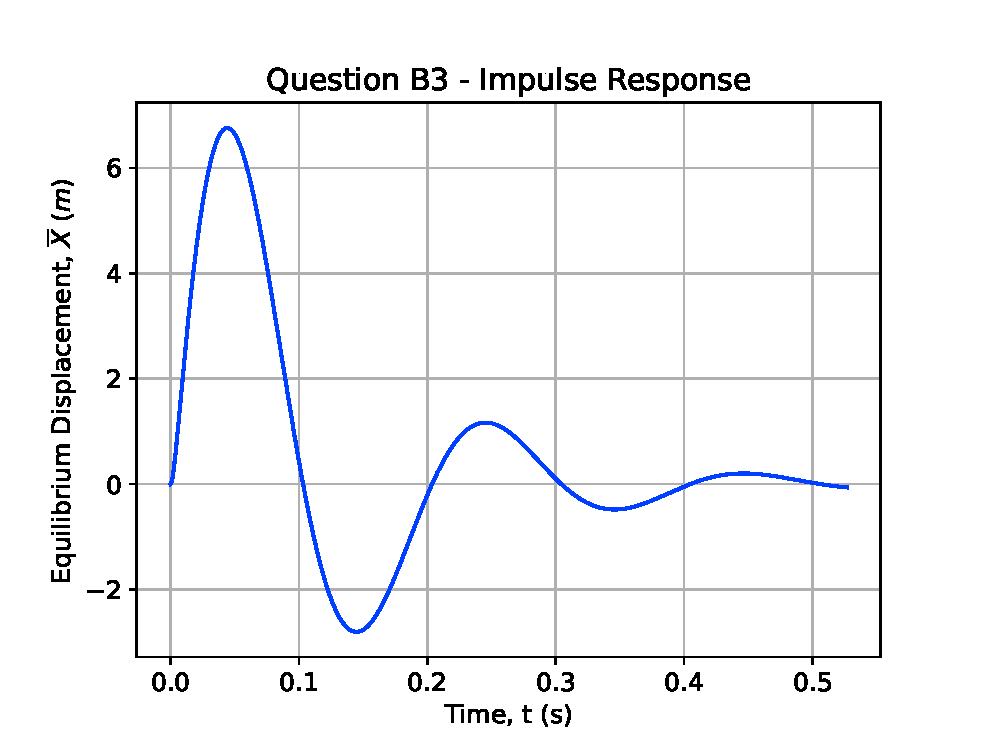
\includegraphics[width=1\linewidth]{Figures/B3_Impulse.eps}
    \caption{Impulse response of the transfer function.}
    \label{fig:B3IDiagram}
\end{subfigure}%
\begin{subfigure}{.5\linewidth}
    \centering
    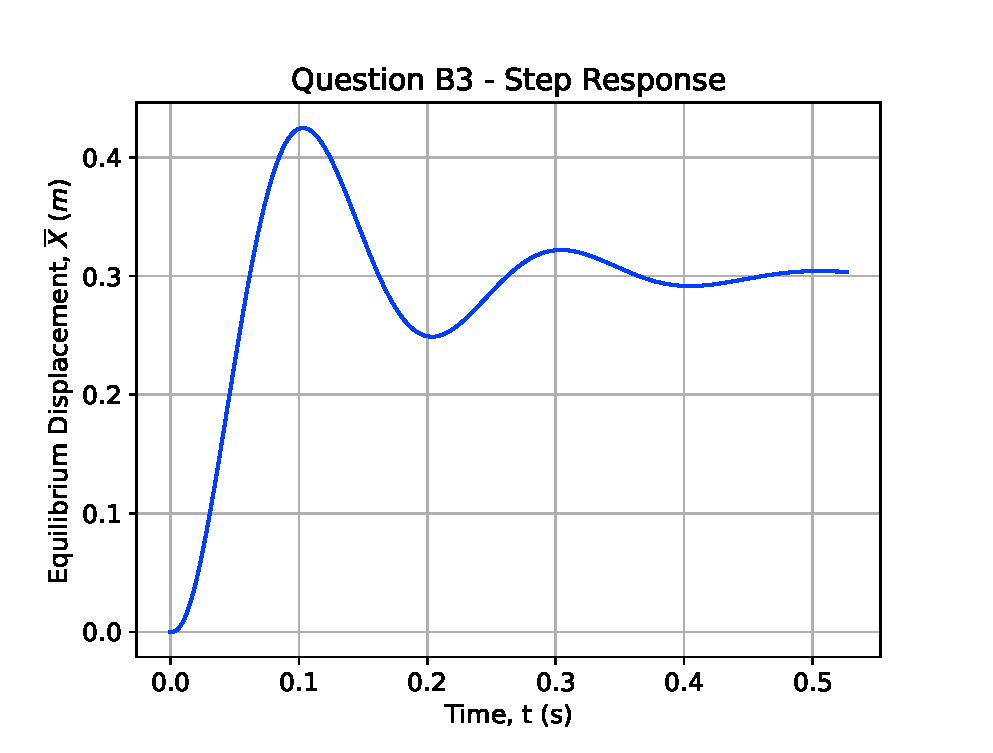
\includegraphics[width=1\linewidth]{Figures/B3_Step.eps}
    \caption{Step response of the transfer function.}
    \label{fig:B3SDiagram}
\end{subfigure}
\caption{Impulse and step response of the transfer function of the linearised system.}
\label{fig:B3Diagrams}
\end{figure}
\par Similarly, to find the step response of the system, $\bar{V}(t)=1$, $\bar{V}(s) = \frac{1}{s}$ and $\bar{z_1}(s) = G(s)\cdot{\bar{V}(s)}$ therefore:
\begin{gather}
    \bar{z_1}(s) = a_1a_4\cdot\bigg(\frac{1}{s+a_4R}\bigg)\bigg(\frac{1}{s^2+a^3s-a_2}\bigg)\cdot\bigg(\frac{1}{s}\bigg)
    \\
    \bar{z_1}(t) = \mathcal{L}^{-1}\bigg\{ a_1a_4\cdot\bigg(\frac{1}{s+a_4R}\bigg)\bigg(\frac{1}{s^2+a^3s-a_2}\bigg)\cdot\bigg(\frac{1}{s}\bigg) \bigg\}
\end{gather}
\par The result of which is shown in figure~\ref{fig:B3SDiagram}.

\subsection{B4 - Bode Plot}
The transfer function of the linearised system facilitates the determination of the the system's frequency response. A program was created in Python, to enable the Bode plot of the frequency response to be plotted. This is presented below:
\begin{figure}[h]
 \centering
 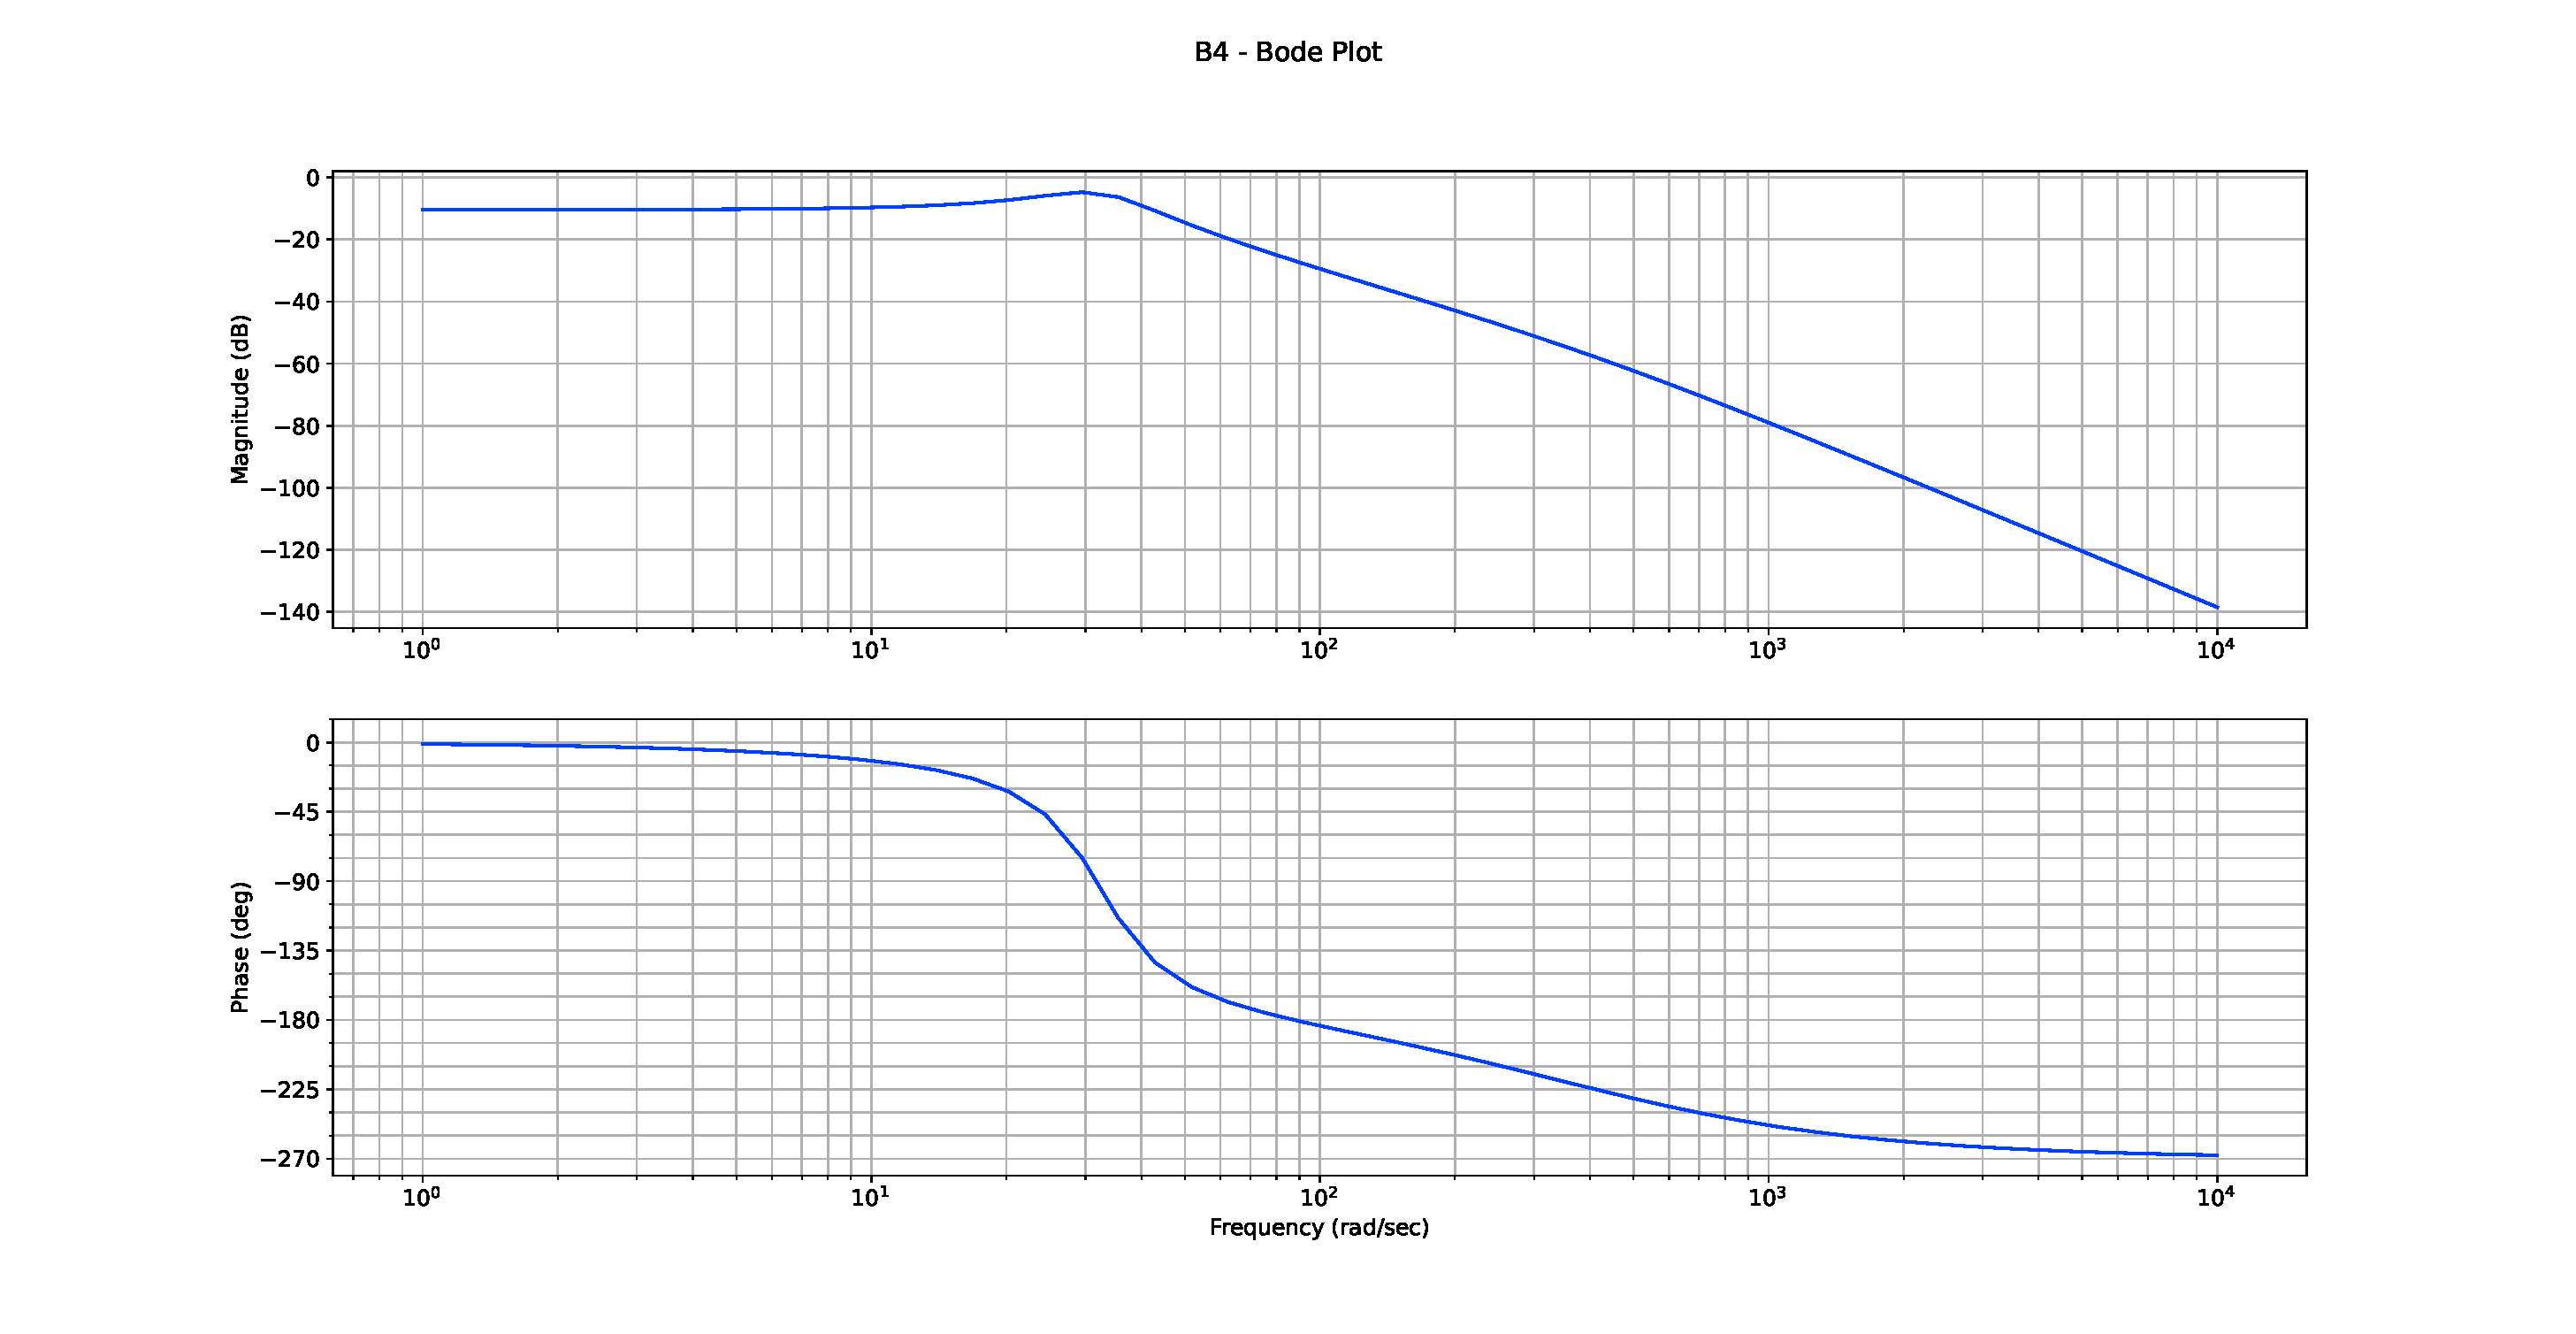
\includegraphics[width=1\linewidth]{Figures/B4_Bode.eps}
 \caption{Bode plot of the transfer function of the linearised system and the frequency response.}
 \label{fig:B4Diagram}
\end{figure}
To determine the low and high frequency asymptotes, the bode graph can be interpreted at the low-end and high-end frequencies separately. From the bode graph, the low frequency asymptote can be approximated as $|Gx(j\omega)|_{(dB)} \approx -10$ and the high frequency asymptote can be approximated as $|Gx(j\omega)|_{(dB)} \approx -10-60\log({\omega})$


\subsection{B5 - Ideal Controller Design}\label{sec:B5}
Supposing that the position of the ball can be monitored using a sensor, an appropriate control system would enable voltage regulation of the electromagnet circuit so to enable the ball to a set-point on the plane. This controller would ideally be able to modulate voltage so that the ball reaches the set-point without oscillation, however, enable the ball to converge to the set-point with an appropriately fast response time. Furthermore, the controller would be able to eliminate any offset present within the system which may have occurred during the modelling of this system. 
\\
\par To determine the suitability of a proposed controller, evidence should be provided demonstrating that the closed-loop system is stable. The expectation of the evidence is that for a range of inputs, the ball does not diverge from the set-point, but instead the ball would converge to the set-point with minimal oscillation and with an adequate response time.\\
\\

\subsection{B6 - Controller Design}
Following the assessment of the desired characteristics of the controller required for the system in section \ref{sec:B5}, implementing a PID controller can be deemed to be a possible approach. The gain values associated to this controller can be tuned to produce the required response; the proportional gain ($K_p$) influences the control action in proportion to the magnitude of the error, which can improve the responsiveness of the system, however may introduce further oscillations to the system; an appropriate derivative gain value ($K_d$), would dampen these oscillations, however increases the response time of the system. Finally, the integral gain ($K_i$) can be utilised to account for any offsets present in the system.
\\

Integrating the PID controller into the system produces the following block diagram:
\\
\begin{figure}[h]
 \centering
 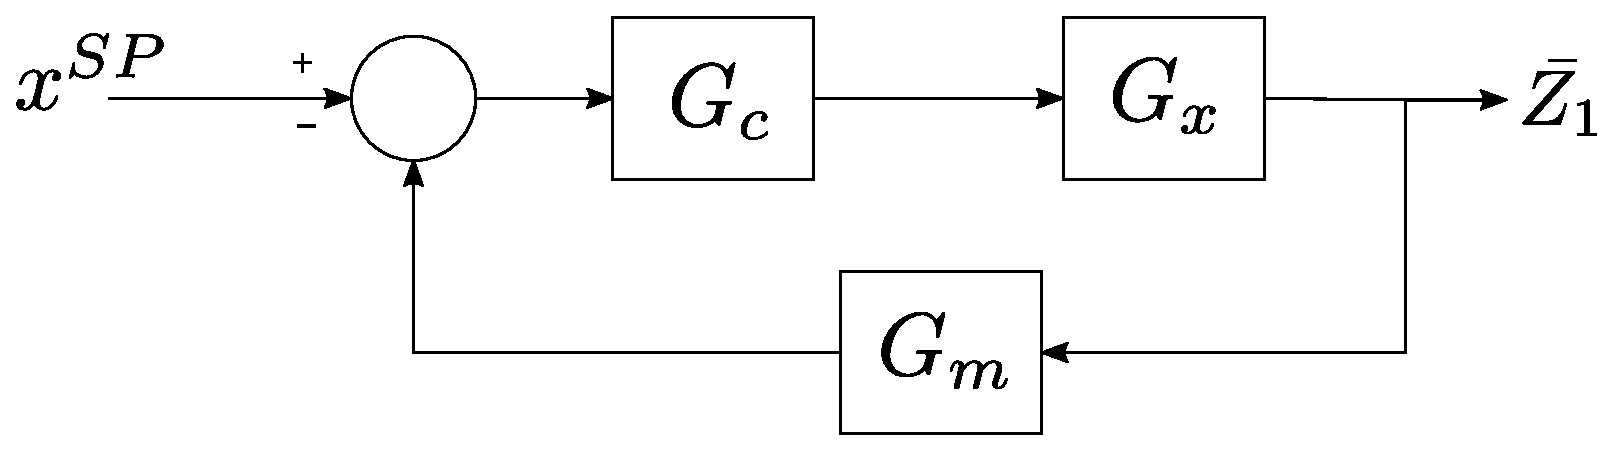
\includegraphics[width=0.8\linewidth]{Figures/Controller_Loop.eps}
 \caption{Block diagram describing the closed loop system.}
 \label{fig:B6Diagram}
\end{figure}
\\
The block diagram describes the composition of the closed-loop system, which can be defined as: \begin{equation}
    G_{cl}(s) = \frac{G_c(s)G_x(s)}{1 + G_m(s)G_c(s)G_x(s)}
\end{equation}
\\
The transfer functions are defined as:
\begin{align*}
    G_c &{}={} \frac{K_ps^2+K_ds+K_i}{s}
    \\
    G_x &{}={} \frac{a_1a_4}{(s+a_4R)(s^2+a_3s-a_2)}
    \\
    G_m &{}={} \frac{1}{0.3s+1}
\end{align*}
\\
where $K_p, K_d, K_i$ are the controller gains and $a1, a2, a3, a4$ are the variables defined by equation \ref{eqn:lin_vars}.

\newpage
\section{Part C}\label{sec:C}

\subsection{C1}
\par Given $f(t) = \ln{t^3}$, $t>0$:
\begin{equation}
    \rightarrow f(t) = 3\ln{t}, t>0
    \notag
\end{equation}

\par Now, Laplace transform of $f(t)$ is

\begin{align}
    F(s) &= \int_0^\infty e^{-st} f(t) \cdot dt
    \notag\\
    &= \int_0^\infty e^{-st} \cdot 3\ln{t} \cdot dt
    \label{eqn:C1Lap}
\end{align}

\par Set $st = u$

\begin{align}
    \rightarrow sdt = du
    \notag\\
    \rightarrow dt = \frac{du}{s}
    \label{eqn:C1s}
\end{align}

\par Inserting ~\ref{eqn:C1s} into ~\ref{eqn:C1Lap}:

\begin{align}
    F(s) &= \frac{3}{s} \int_0^\infty e^{-u} \cdot \ln{\bigg(\frac{u}{s}\bigg)} \cdot du
    \notag\\
    &= \frac{3}{s} \int_0^\infty e^{-u} \cdot \ln{u} \cdot du - \frac{3}{s} \int_0^\infty e^{-u} \cdot \ln{s} \cdot du
    \notag\\
    &= \frac{3}{5}(-\gamma) - \frac{3}{5}\ln{s}\bigg[\frac{e^{-4}}{-1}\bigg]_0^\infty
    \notag\\
    &= \frac{3}{5}(-\gamma) - \frac{3}{5}\ln{s}[0+1]
    \notag\\
    &= -\frac{3}{5}\bigg(\ln(s) + \gamma\bigg)
    \notag
\end{align}
\\
\par Where $\gamma$ is the Euler's constant. Therefore, the Laplace transform of $f(t)$ is:

\begin{equation}
    -\frac{3}{5}\bigg(\ln(s) + \gamma\bigg)
\end{equation}

\newpage
\section{Part D}

\subsection{D1 - Collaboration}
\par Throughout this project, a \href{https://github.com/Lorcan-Q/Control_Coursework}{Github repository} was utilised. Collaboration on the \LaTeX\;file was possible through Overleaf, which enabled concurrent access to the report while also providing its own source versioning system. Unfortunately due to group participation, the workings and code for the problems were created and uploaded by Lorcán alone; however, Toby ensured his participation through the generation of the report and peer reviewing this work. Tasks and responsibilities were initially shared amongst the team, to provide multiple insights to the correct function of the system; however as previously mentioned, this devolved during the latter stages of the project. An issue tracker was created at the beginning of this project, however as the project progressed, Microsoft Teams meetings were used to communicate issues and for simultaneous work.

\subsection{D2 - Functioning as a team}
\par The final team members provided good communication with each other, provided through daily meetings to discuss progress and issues. Furthermore, the Github repository and collaborative features on Overleaf enabled efficient peer review of our progress and enabled us to provide any assistance necessary.  When completing the \LaTeX\;file, members collaborated by simultaneously working on the file and resolved issues and improved sections when provided with a different view point.


\subsection{D3 - Challenges and issues}
\par Unfortunately, due to COVID-19 the dynamic of the group project was difficult; however, the use of the Github repository enabled completed workings to be shared to team members and meetings on Microsoft Teams enabled good communication. Another issue encountered was the lack of participation from a member within the group however to ensure the completion of the project, the workload was shared amongst the remaining members.\\
\\
PLEASE NOTE: On the day of the deadline, we received contact from our team member Syed. Despite not partaking in the group's completion of the project, Syed provided workings to the bonus questions completed in section \ref{sec:C}. 

\end{document}
